\chapter*{Introduction}
\addcontentsline{toc}{chapter}{Introduction}

\section*{Goal}

Source code documentation is an essential part of any quality project. Writing, and keeping such documentation up to date is often overlooked, or too cumbersome to do, due to a variety of reasons, such as strict deadlines. This might lead to the degradation of project quality, as developers who leave said projects usually take their know-how with them without properly passing them down to their replacements.

In cases where source code documentation has a higher priority than usual, it is also considered good practice to extract said documentation from the source code into a searchable, public format such as \ref{itm:html}. This is accomplished with documentation generating tools. The primary benefit of this practice is the resulting comprehrensive overview of the source code, which can be easily shared with interested parties.

For Microsoft \ref{gloss:dotnetlabel} projects there is a selection of documentation generating tools available, which includes: DocFX, Doxygen, SourceBrowser, and others. These solutions primarily generate output in \ref{itm:html}, which is sufficient for the majority of projects. However, most of them lack in support for other output formats like \ref{itm:pdf}, \ref{gloss:markdown}, or custom formats. Moreover, customization of these tools is very limited, which prevents projects from being able to fit such tools to their exact needs. More often than not, said tools lack in \ref{itm:ui}/\ref{itm:ux} areas, introducing an unnecessary learning curve and lowering usability.

With that in mind, there is visible room for improvement. A desirable documentation generating tool would be easy to use, modern, extensible, rich in output format support, and performant. Satisfying the desires of an extensible modern application requires thorough use of programming design patterns such as \ref{itm:solid}, \ref{itm:di}, and \ref{itm:mvvm}.

Thus, the goal of this thesis is to create a custom documentation generating tool for \ref{gloss:dotnetlabel} projects using common design patterns such as \ref{itm:solid}, \ref{itm:di}, and \ref{itm:mvvm}, and to satisfy user needs for extensibility, ease of use, modern design, and support for many output formats. All of this has to be achieved without introducing worse performance than existing toolst.

\section*{Motivation}

The motivation for creating a custom tool is primarily a personal need to provide easy access to code documentation. Since most open source projects are hosted either on GitHub.com\footnote{A Microsoft-owned Git hosting platform} or GitLab.com\footnote{An independent Git hosting platform}, it makes sense to utilize said platforms built-in wiki pages for hosting source code documentation for consistency. A minority of developers use Bitbucket\footnote{TODO} to host their public open source projects as this platform is predominantly used in the enterprise market. Additionally, corporate clients who purchase Bitbucket usually purchase Confluence alongside it, which serves as a documentation hosting platform. With this in mind, directly supporting Bitbuckets wiki is not a priority; however, adding future support for confluence is possible, given the extensibility of the tool.

When attempting to find existing solutions for generating documentation, none had the desired extensibility and were mainly limited to only creating static \ref{itm:html} pages
\footnote{A static web page is a page that is built using \ref{itm:html} code and features the same presentation and content, regardless of user identity or other factors \cite{techopedia_what_2017}}.
Since major \ref{gloss:git} hosting platforms wiki pages predominantly utilize \ref{gloss:markdown} for displaying formatted text\footnote{Apart from \ref{gloss:markdown}, said \ref{gloss:git} platforms support more formats; however, the latter has the richest formatting capabilities}, static \ref{itm:html} pages are out of the question.

And so, the idea to develop a custom tool that would create \ref{gloss:markdown} documentation from \ref{gloss:dotnetlabel} libraries for \ref{gloss:git} platforms came to fruition. Nevertheless, focusing only on one output format would be a waste of time and effort, as few to none would need such a tool. Thus, the result of the development should be a generic tool that allows anyone to modify it to output to any desirable format.

To backup this motivation, a questionnair had been conducted to identify developer needs for documentation generating tools in the \ref{gloss:dotnetlabel} world. The result of the questionnair (see \ref{sec:whatdouserswant}) confirmed general low interest in writing documentation; however, it highlighted the desires of those few developers who do care about maintaining source code documentation.

With that in mind, it is clear that the target group for such a tool is minor. Given that, focusing on the extensibility feature of the tool is crucial to cover thir needs.

\section*{Strategy}

What follows are milestones for the project development.
Achieving each one is a step closer to the end goal of a functioning custom documentation-generating tool.

The basis for said milestones is on the analysis of current documentation tools (see \ref{sec:whatisavailable}), the developer needs (see \ref{sec:whatdouserswant}), personal experience, and general project development guidelines.

\subsection*{Proof of concept} \label{subSecProofOfConcept}

Creating a proof of concept program will help understand whether the project is realistic, what challenges will occur and how to overcome them.
The main drawback of this is that it will take additional time; however, the gained perspectives are quintessential for the correct planning of the project.

The main focus of this milestone is to find out how to extract the necessary data for documentation generation and attempt to generate said documentation.
This is needed because no other reliable reference project was found that could provide required guidelines in a reasonable amount of time.
All other requirements based on the takeaways from the survey (see \ref{ssec:questionnaireeval}) can be omitted from this stage, as reference projects and personal experience is available.

\subsection*{Evaluations and project planning} \label{subSecEvalProjPlanning}

Concise planning of the project, based on the gained experience from the proof of concept, will, as a result, yield a higher quality product.
Extensibility will be the key feature of the project. Careful planning of the code structure is required to avoid unnecessary complications.
Meanwhile, the planning phase shouldn't take unreasonable effort, as the ratio of time spent to results will diminish over time (as seen in \ref{fig:overplanning}). \cite{ruparelia_stop_2016}

\begin{figure}[H]
    \centering
    \caption{Overplanning visualized}
    \label{fig:overplanning}
    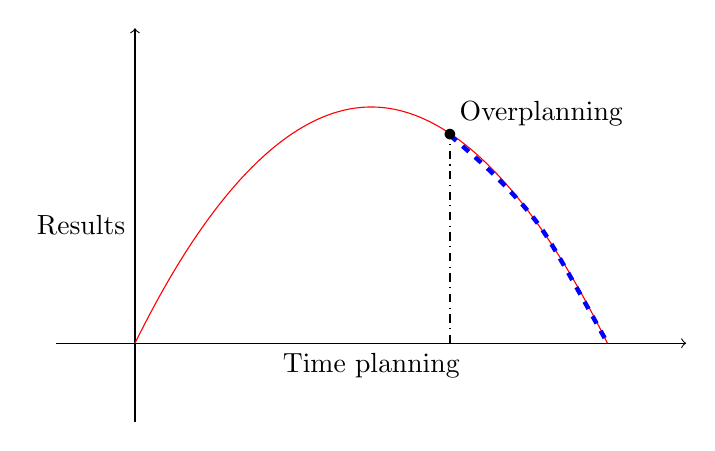
\begin{tikzpicture}
        \draw [->] (-4, 0)--(4,0) node [midway, below]{Time planning};
        \draw [->] (-3, -1)--(-3,4) node[left, midway]{Results};

        \draw [red] (0, 3) parabola(-3,0); % Left
        \draw [red] (0, 3) parabola(3,0); % Right
        \draw [ultra thick, blue, dashed] plot [smooth] coordinates {(1, 2.64) (1.6,2.1) (2.2, 1.40) (3, 0)}; % Right

        \draw [dash dot] (1,0)--(1, 2.64);

        \draw (1, 2.64) node [above right]{Overplanning};
        \draw (1, 2.64) node {$\bullet$};
    \end{tikzpicture}
\end{figure}

The goal of this milestone is to gain a clear picture of what techniques, design patterns, and technologies should be used or avoided to satisfy all prject requirements with minimum compromise.

\subsection*{Basic structure} \label{subSecBasicStructure}

Setting up the project structure and introducing interfaces will pave its foundation. The resulting project structure should cohere with the plan from the previous milestone.

Ensuring minimum coupling of interfaces will be the priority of this milestone, as it will maximize the modularity of the parts composing the project.
Other goals include:
\begin{itemize}
    \item Setting up a \ref{itm:cicd} build environment
    \item Documenting the interfaces
    \item Preparing an empty test console application for the next milestone
\end{itemize}

\subsection*{Processing libraries} \label{subSecProcessingLibs}

The focus of this milestone will be the creation of working processing libraries that will serve as the core of the application. Said libraries will take some input and generate documentation as an output. The types of libraries and their implementation depend on the previous milestones. The result of this milestone will be a set of working libraries testable via a console application.

\subsection*{GUI application} \label{subSecGuiApp}

The \ref{itm:gui} application will serve as the façade to users utilizing the tool. Said application must be cross-platform, have a modern design, and provide as seamless a user experience as possible, considering the extensible nature of the tool.

Thus, the goal of this milestone is to create such a \ref{itm:gui} façade that will have a simple, yet functional \ref{itm:ux}/\ref{itm:ui}. Additional goals might be added based on the outcomes of previous milestones.

\subsection*{Markdown for Git plugin} \label{subSecMdGitPlugin}

Creating the first plugin for the tool will be the final milestone for the time being, as after its creation the goal of this thesis is reached.
The plugin will be composed of the processing libraries created in the fourth milestone.

The goal is to create such a plugin, that can be distributed separately from the main application. This would allow users to choose what plugins they wish to use, and omit installing ones they don't.
